After the creation of the dense point cloud, we can use metashape to create a polygonal mesh model with the point cloud information and the the depth maps data. The \emph{build mesh} command used to create a mesh for the selected point cloud. To get a high quality output we selected the source data to be the dense point cloud, even though it requires a longer processing time. The face count specifies the number of polygonals in the final we used the high settings in our reconstruction to give a quality mesh. The vertex colors are calculated and the depth maps from the alignment process is reused here.\\

\begin{figure}[H]
	\centering
	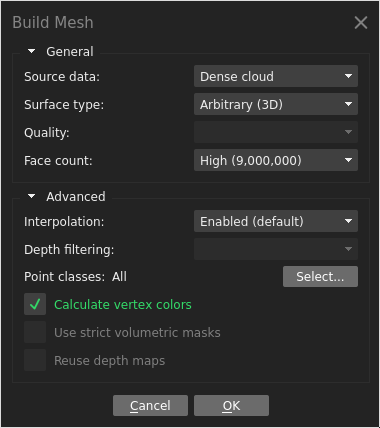
\includegraphics[scale=0.5]{img/mesh.png}
	\caption{Mesh Generation}
\end{figure}
Texture genration in metashape uses the source data from the aligned images which allows it build a color texture map for the model. Metashape also allows to fill holes in the model. We kept the other parameters same as the default standard when building the texture. The texture model that we obtained from metashape had higher quality but they occupied more space with higher the quality.

\begin{figure}[H]
	\centering
	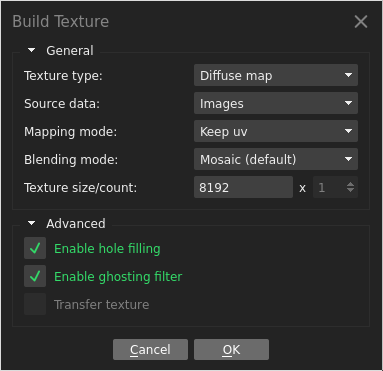
\includegraphics[scale=0.5]{img/texture.png}
	\caption{Texture Generation}
\end{figure}

%[1](https://www.agisoft.com/pdf/metashape-pro_1_8_en.pdf)
